\chapter{GEM Detector Data Analysis}

Gas Electron Multiplier (GEM) detector is one kind of gaseous detector. At the heart of these detectors is a 5 µm copper-coated polyimide foil, which is punctured with 70 µm holes in a regular hexagonal pattern, spaced 140 µm apart. The GEM foil features a cathode on top, while a readout board is situated beneath it for collecting the electrons generated during the ionization process. When a potential difference is applied across the foils, it produces sharp electric fields within the holes, which multiply the electrons and result in an electron avalanche. This avalanche electrons travels along the electric field and is eventually collected by the finely spaced strips. To enhance amplification, multiple GEM detector layers are stacked together, allowing ionized electrons to be amplified multiple times before reaching the readout board.

The GEM detectors utilized in the PRex/CRex experiment were specifically designed for the Jefferson Lab Super BigBite Spectrometer (SBS) and span an area of 50 cm x 60 cm. At the time of its construction, it was one of the largest GEM detectors ever built. The PRex/CRex experiment offered an excellent opportunity to test the GEM detector in a real experimental environment before initiating the SBS experiment. The detector serves as a valuable supplement in situations where the event rate is high, as the VDC efficiency declines or even fails under such conditions. This chapter delves into the apparatus and the analysis results of the GEM detectors.

\section{GEM Detector Configuration}

The SBS GEM detector used in the PRex/CRex experiment comprises three layers of GEM foils. The cathode, situated on top of the GEM foil, features a similar hole structure but is single-side coated instead of double-sided. To prevent polarization due to charge accumulation on the cathode, a thin aluminized gas window layer is applied, which shares the same high voltage as the cathode.

A premixed gas containing $75\%$ Argon and $25\%$ Carbon Dioxide is supplied by the Hall A gas system for use in the GEM detector. This mixed gas first enters the chamber between the entrance window and the cathode, then passes through the holes in the foil, ensuring a uniform gas mixture throughout the entire chamber. Exhaust gas exits through exhaust holes located on the frame at the bottom of the GEM chamber.

At the base of the GEM foils, avalanche electrons are collected by 2D readout strips. Each readout strip is connected to a charge-sensitive pre-amplifier electronics channel. To counteract any bending of the readout board due to the mixed gas in the chamber, an additional chamber is designed beneath the readout board and filled with air at the same pressure as the GEM chambers.


\begin{figure}[!tbp]
  \centering
  \begin{minipage}[b]{0.45\textwidth}
    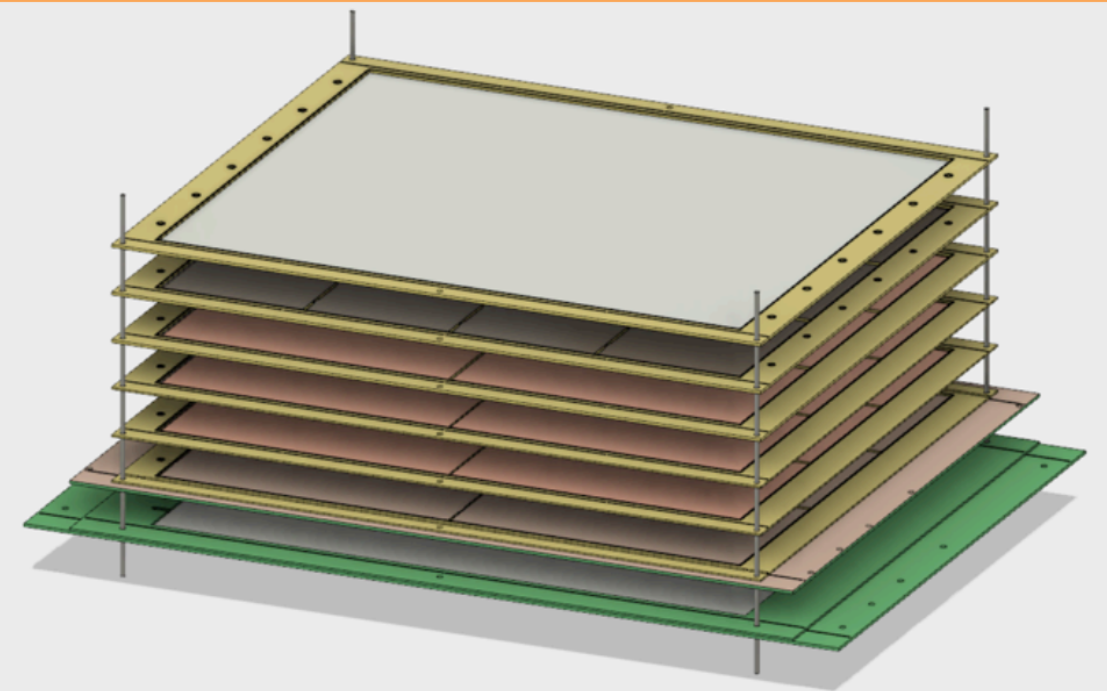
\includegraphics[width=\textwidth]{images/chap5/gem_structure_3d.png}
    \caption{GEM Chamber 2D structure}
  \end{minipage}
  \hfill
  \begin{minipage}[b]{0.45\textwidth}
    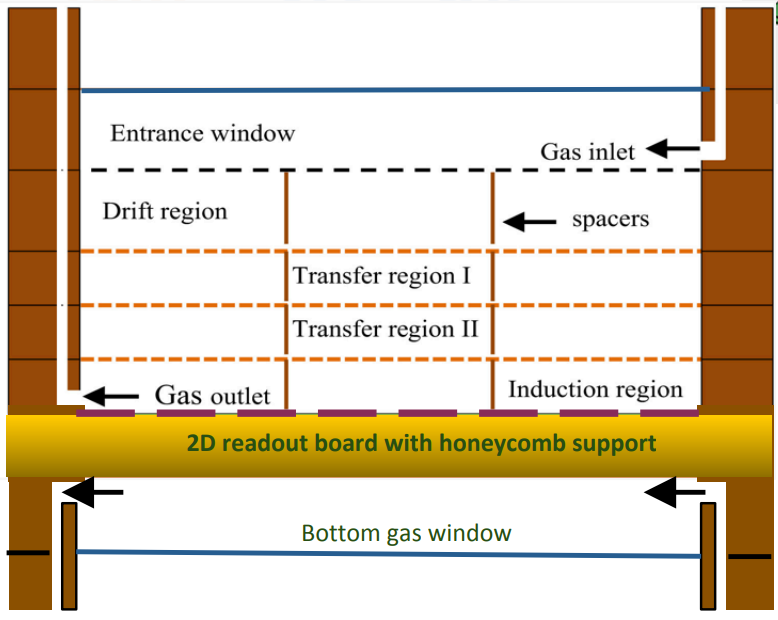
\includegraphics[width=\textwidth]{images/chap5/gem_structure_chamber_2d.png}
    \caption{GEM chamber Gas flow}
  \end{minipage}
\end{figure}


\subsection{GEM detector in Hall A High-Resolution Spectrometer}

Each HRS have 3 SBS GEM detectors with the size of $50cm x 60cm$ and 3 smaller sizes GEM detector with the size of $10cm x 20cm$ manufactured by Idaho State University. As shown in the figure, the GEM detectors are parallel to each other, placed after the VDC detectors.  The Idaho GEM detectors are placed in front of the SBS gem detectors. Two quartz detectors are placed in between the first and the second Idaho GEM detectors, and another two AT detectors are placed between the SBS GEM detectors and the Idaho GEM detectors. 


\begin{figure}[!htbp]
  \centering
  \begin{minipage}[b]{0.45\textwidth}
    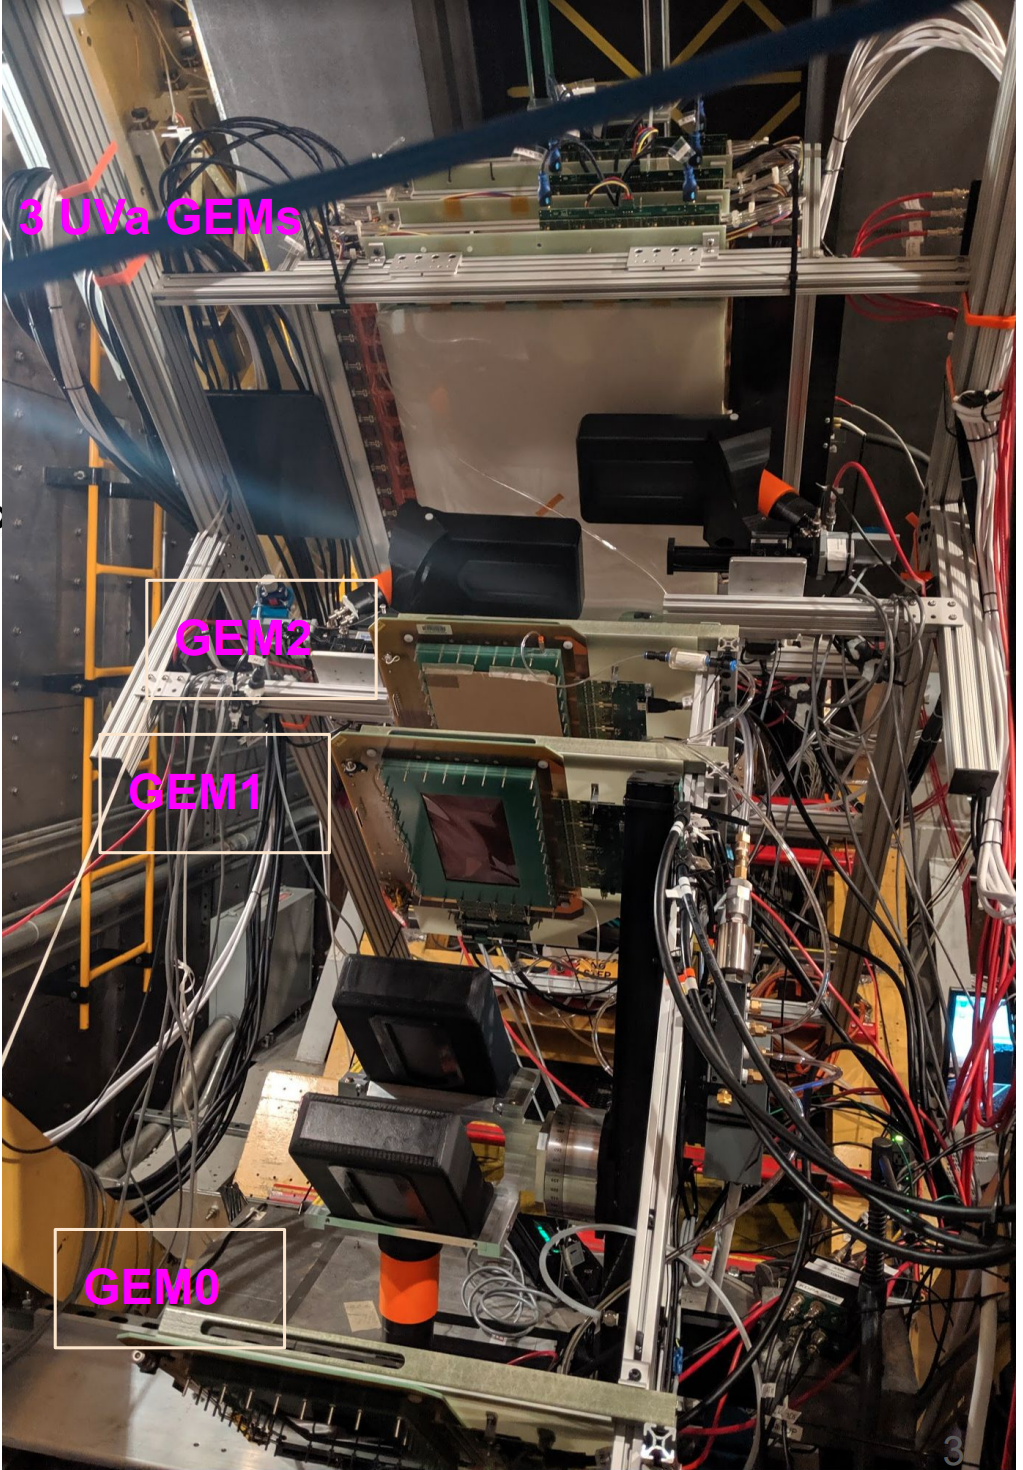
\includegraphics[width=\textwidth]{images/chap5/gem_in_apparatus_photo.png}
    \caption{GEM Chamber 2D structure}
  \end{minipage}
  \hfill
  \begin{minipage}[b]{0.45\textwidth}
    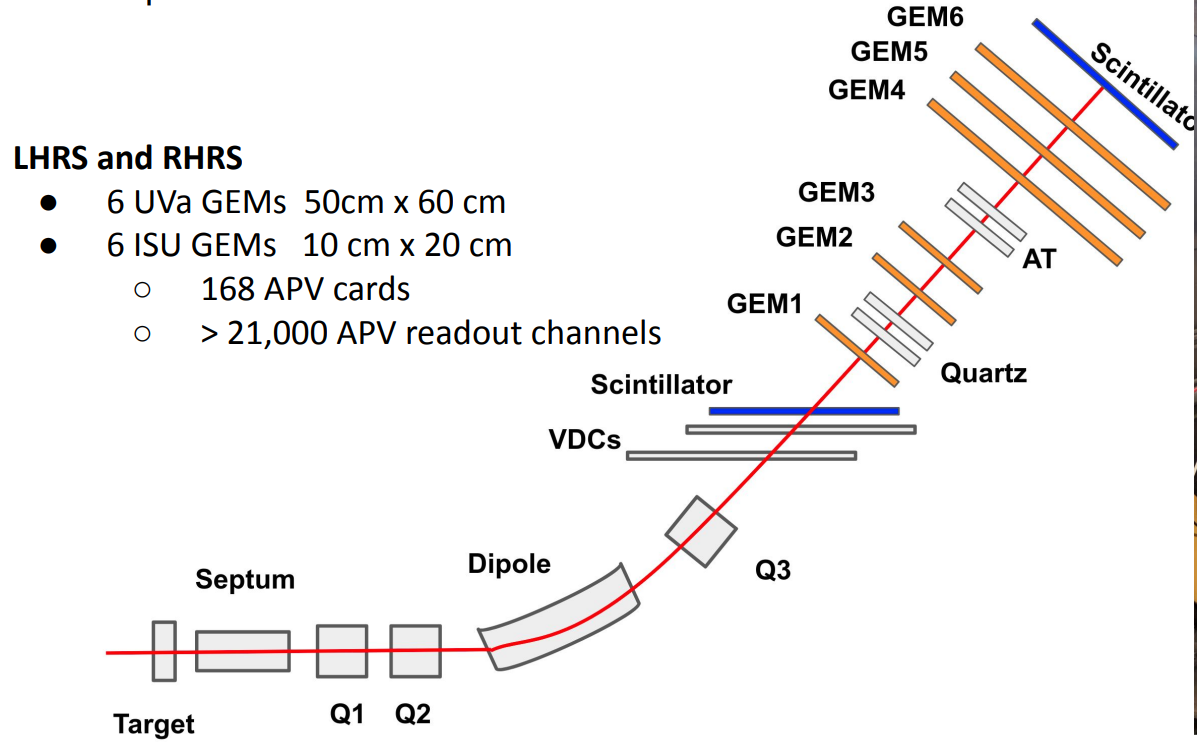
\includegraphics[width=\textwidth]{images/chap5/gem_apparatus_in_hrs_2d.png}
    \caption{GEM chamber Gas flow}
  \end{minipage}
\end{figure}


\subsection{Add a more detailed introduction of GEM detector supplement electronics??}
\begin{enumerate}
    \item readout electronics (APV, MPD, CPU, coda)
    \item low voltage for the APV (modular LV, cable selection, LV regulator, cooling fan) 
    \item High Voltage
    \item Gas System
\end{enumerate}


\begin{figure}[!htbp]
  \centering
  \begin{minipage}[b]{0.45\textwidth}
    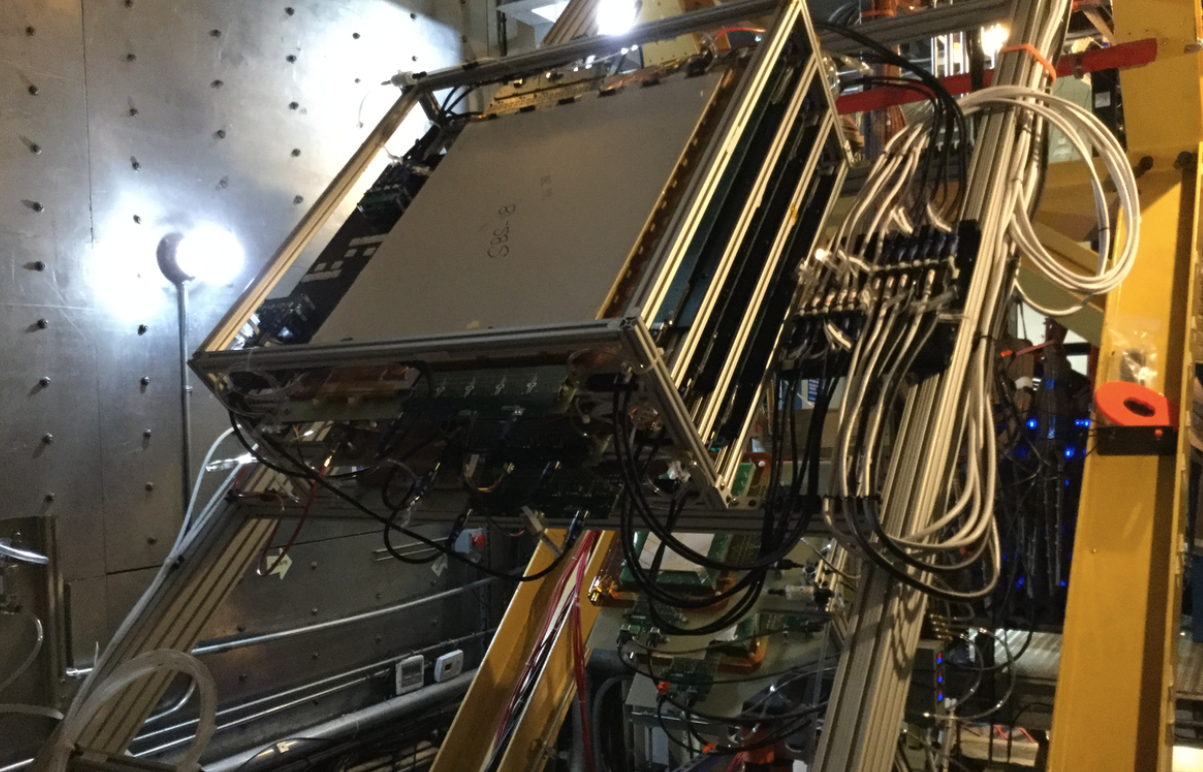
\includegraphics[width=\textwidth]{images/chap5/gem_in_hrs.png}
    \caption{GEM Chamber in HRS}
  \end{minipage}
  \hfill
  \begin{minipage}[b]{0.45\textwidth}
    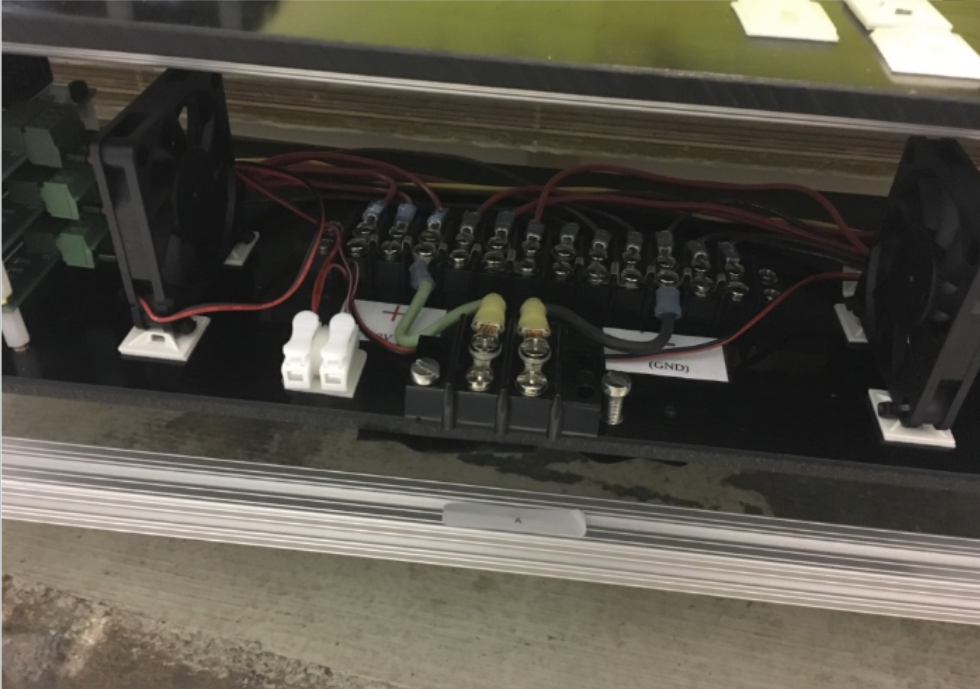
\includegraphics[width=\textwidth]{images/chap5/gem_low_voltage.png}
    \caption{GEM Pre-Amplifier Voltage Supply}
  \end{minipage}
\end{figure}


\begin{figure}
    \centering
    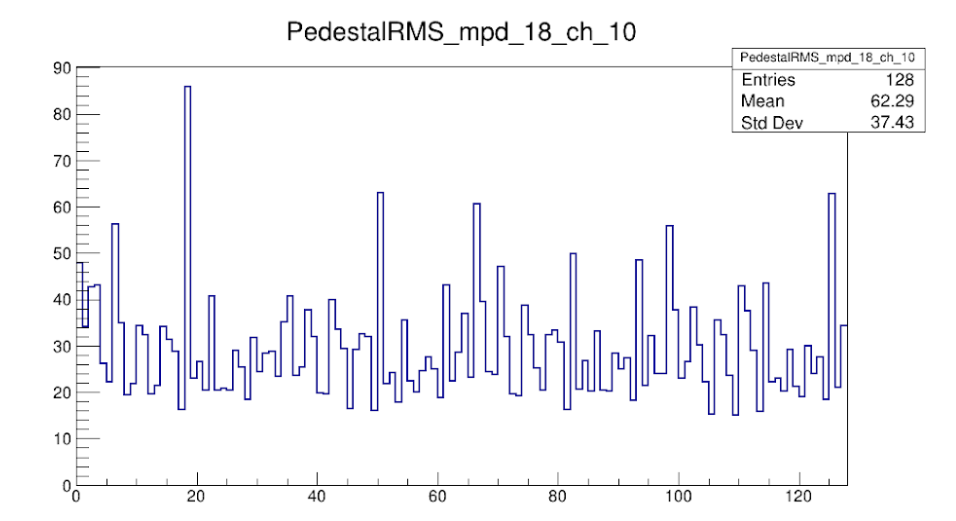
\includegraphics[width=\textwidth]{images/chap5/gem_signal.png}
    \caption{Caption}
    \label{fig:apv_25_pedestal_plot}
\end{figure}


\begin{figure}
    \centering
    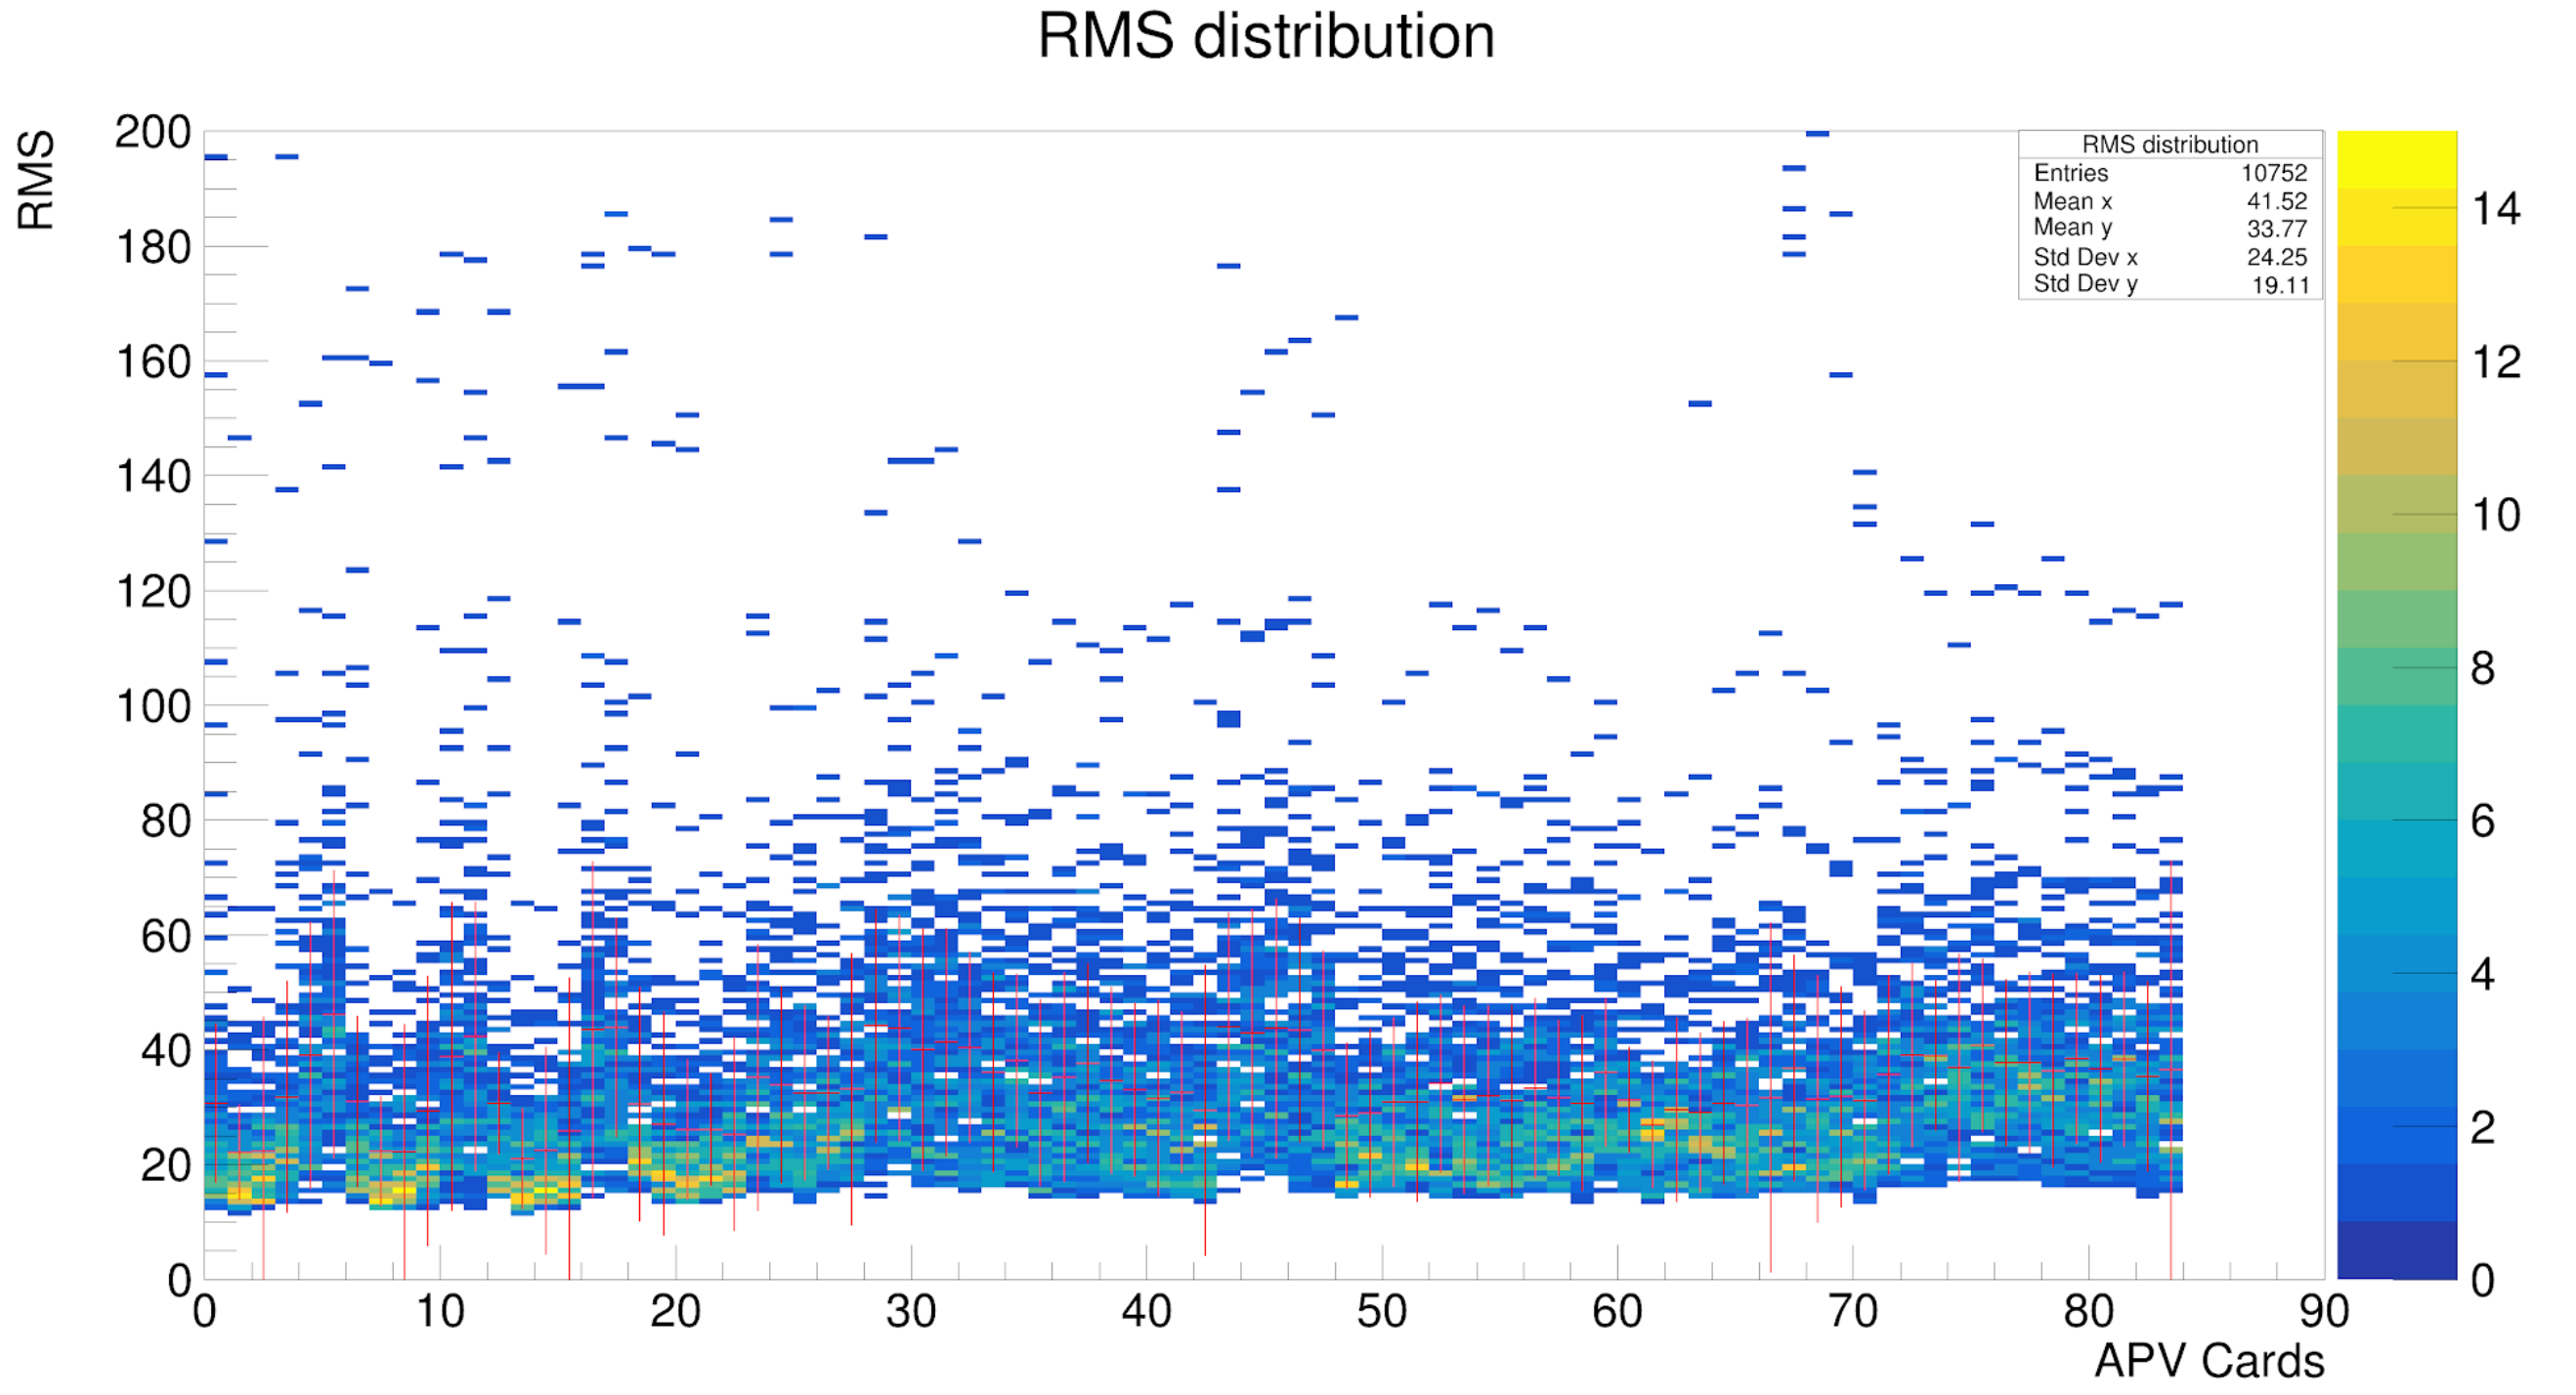
\includegraphics[width=\textwidth]{images/chap5/LHRS_pedestal.png}
    \caption{Caption}
    \label{fig:my_label}
\end{figure}

\begin{figure}
    \centering
    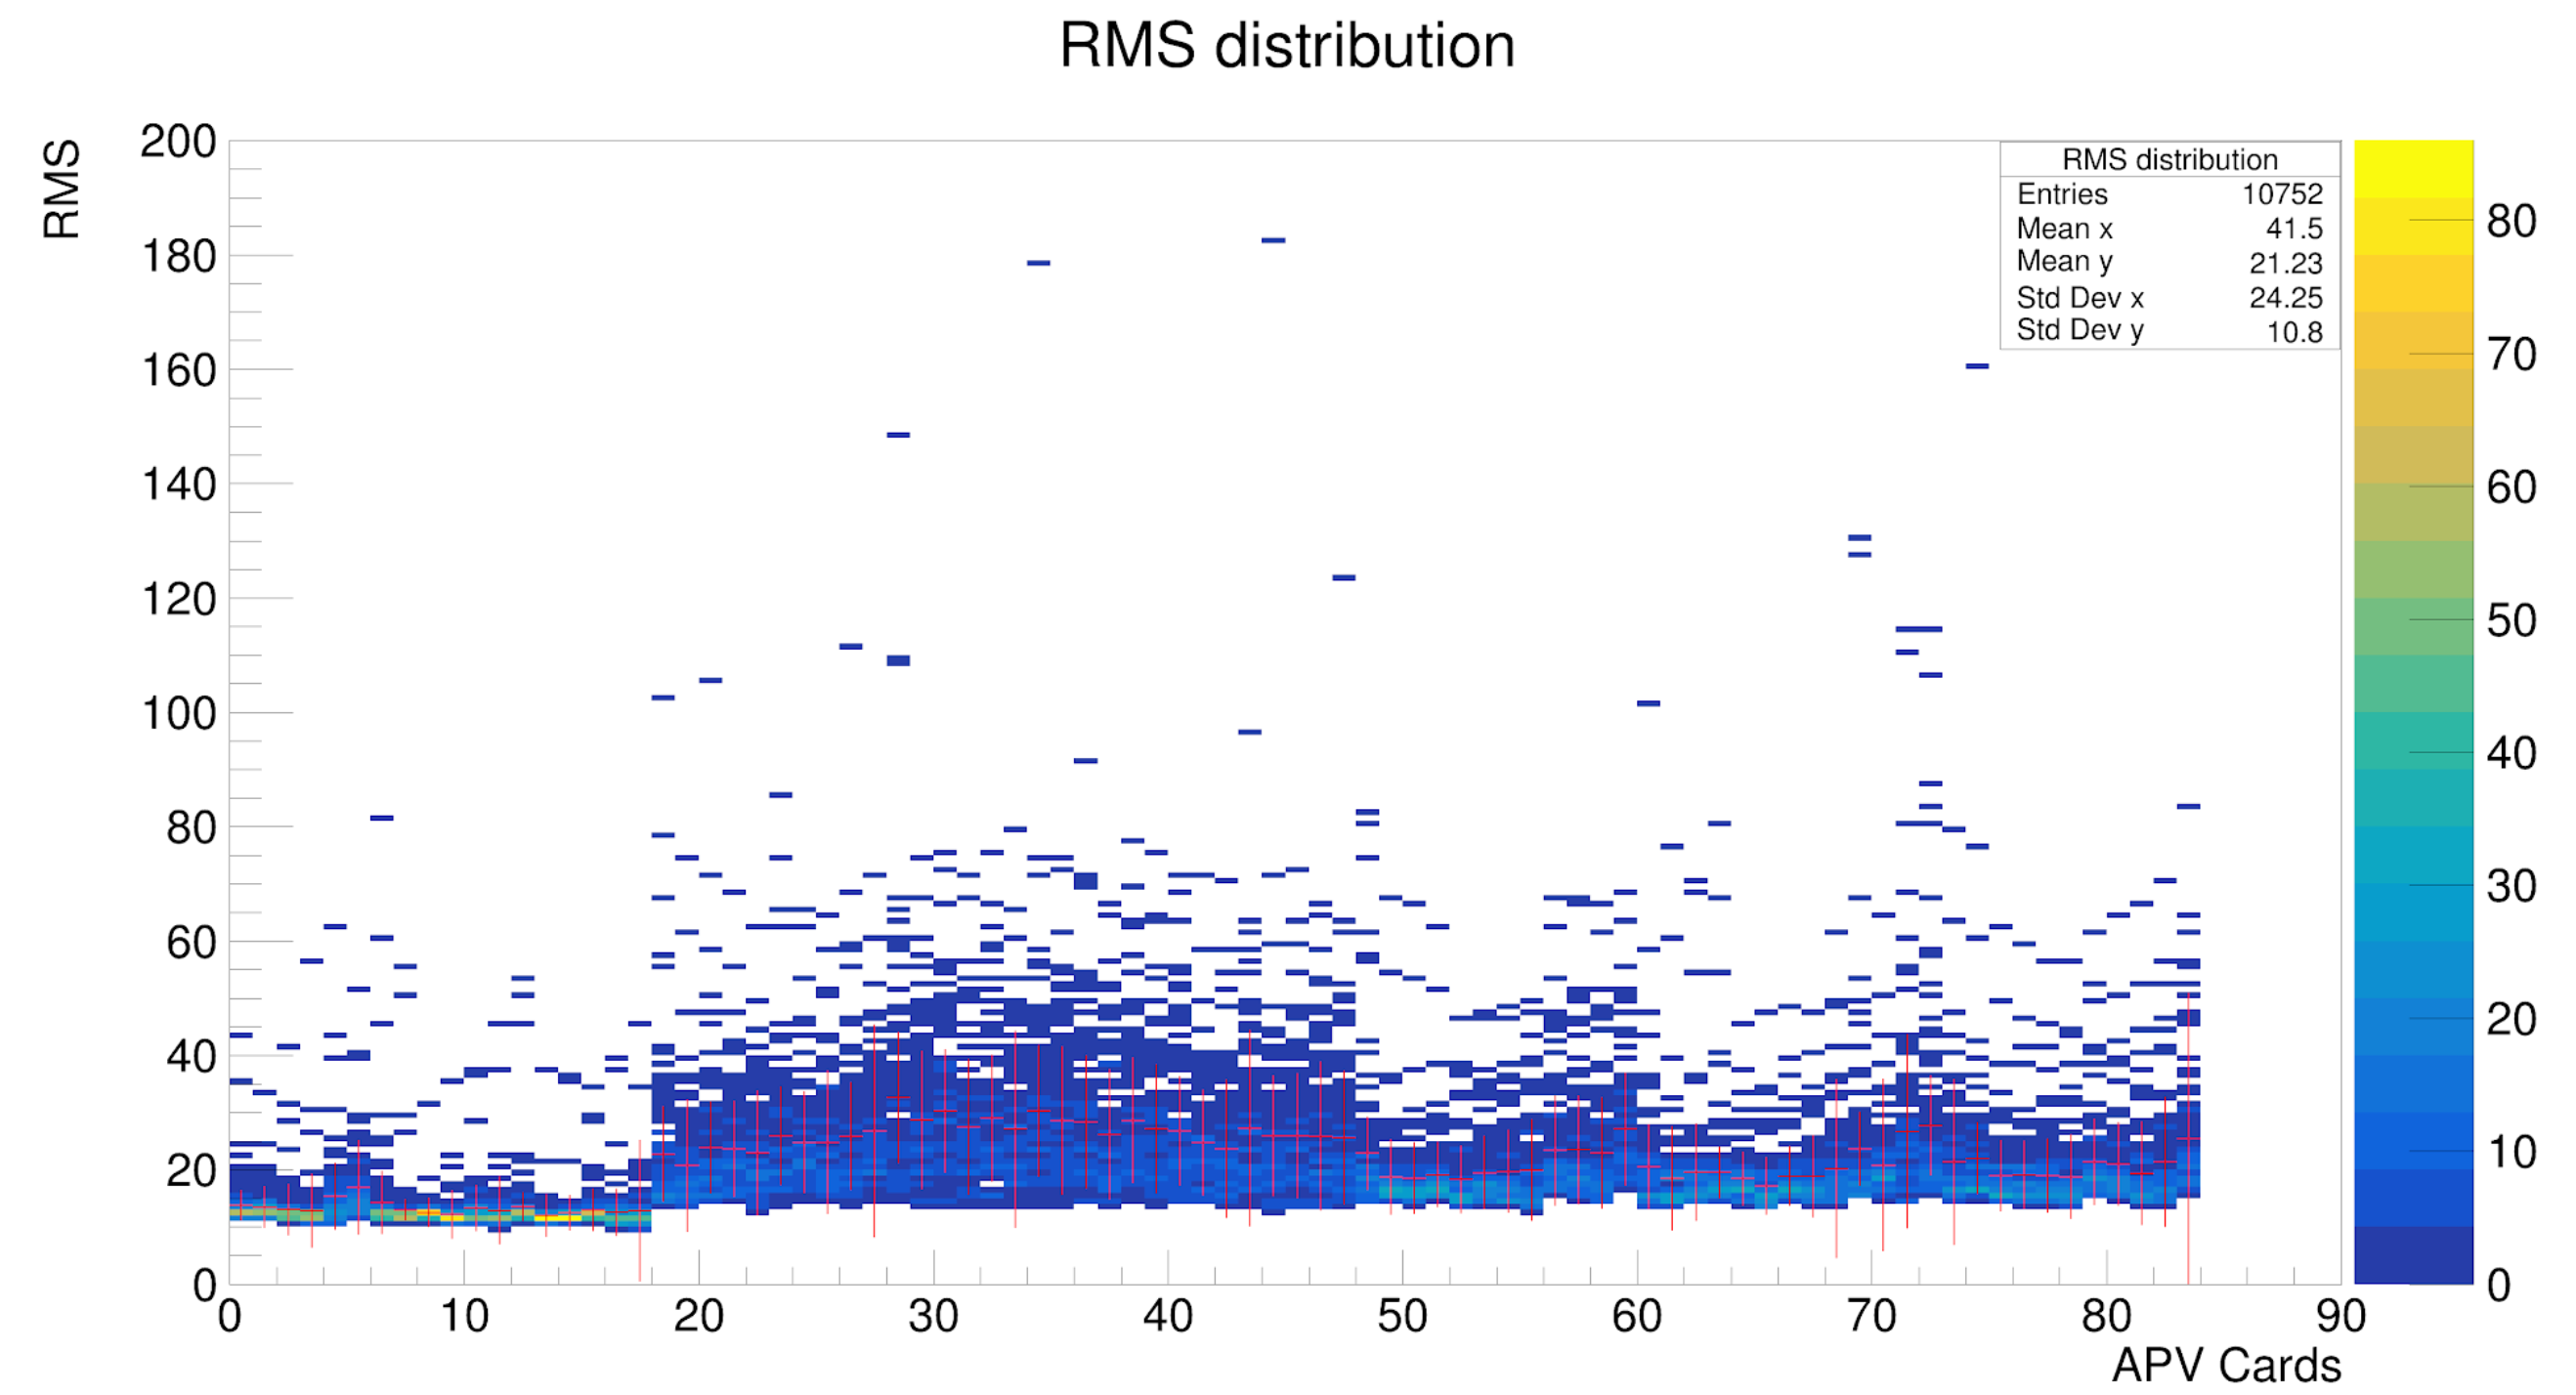
\includegraphics[width=\textwidth]{images/chap5/rhrs_pedestal.png}
    \caption{Caption}
    \label{fig:my_label}
\end{figure}


\begin{figure}
    \centering
    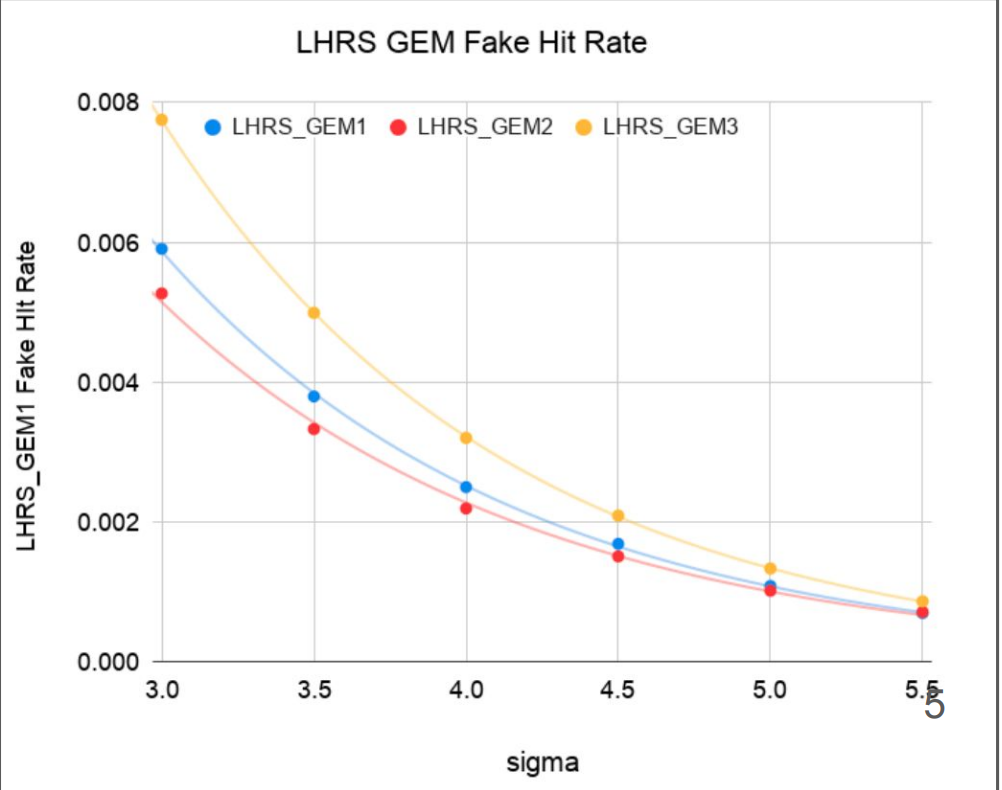
\includegraphics[width=\textwidth]{images/chap5/lhrs_fake_hit_rate.png}
    \caption{Caption}
    \label{fig:my_label}
\end{figure}


\begin{figure}
    \centering
    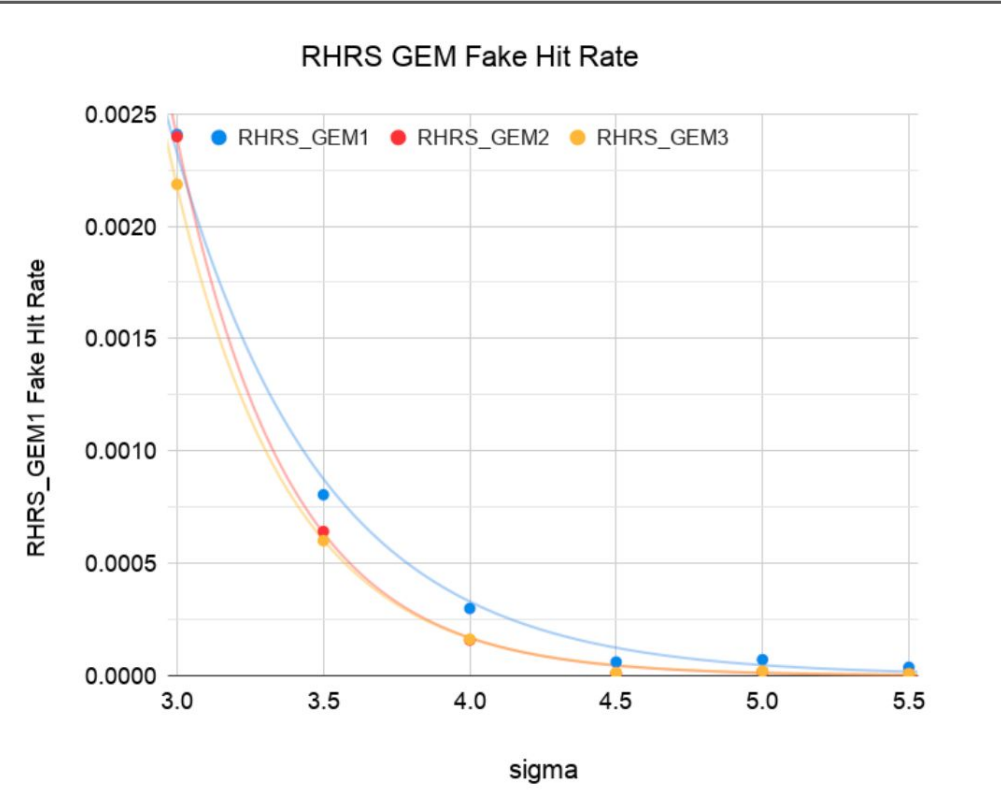
\includegraphics[width=\textwidth]{images/chap5/rhrs_fake_hit_rate.png}
    \caption{Caption}
    \label{fig:my_label}
\end{figure}

\section{GEM detector data analysis}
The GEM detector readout strips are connected to the APV frontend card, which is a 128-channel pre-amplifier. The signal after APV is sent to Multi-Purpose Digitizer where it converts to digital signals with 12-bit Analog to Digital converter.  Figure \ref{fig:apv_25_pedestal_plot} shows a typic plot after the MPD. The X-axis is the APV channels, while as the Y-axis is the ADC values after the ADC converter which is proportional to the number of charges collected by the given strip. 



\subsection{the procedure used to get the GEM signals}
\subsection{pedestal}
\begin{itemize}
    \item how to get the pedestal
    \item pedestal False Positive Rate Study
\end{itemize}
\subsection{GEM detector alignment}
\subsection{GEM detector performance}
\begin{itemize}
    \item GEM detector cluster size
    \item GEM detector number of strips fired
    \item GEM detector tracking efficiency
    \item GEM detector efficiency over time 
    \item GEM detector High Rate Performance and compare with VDC 
\end{itemize}
